\section{Application functionality}
\subsection{Account management}
A user needs to be identified uniquely, and that is done through an Ethereum\glo account. The functions uploaded will be linked to your account, and the execution fees will be detracted from the same account. Also, each Ethereum\glo network call, will consume gas and as a consequence, you will need log in before using all functionalities.\\\\An Ethereum account is not identified by the same means as an usual account (eg. name, email), but by an address and private key which are not user-chosen but assigned by the network when requested.
\\\\
Once a user is logged, a session is created and it lasts until the user logs out. To keep the session data safely stored, we encrypt locally your credentials with a password. When a command that needs the account private key is called, the password should also be provided.
%To have access to the application, use the following  command to view the list of all commands with a short description:\\\\
%\centerline {\code{etherless init}}
%\begin{figure}
%	\centering
%	\includegraphics[width=\textwidth]{res/img/Screenshot_init.jpg}
%	\caption{command list}
%\end{figure}
\subsubsection{Registration}
To generate a brand new Ethereum account use the following command:\\\\
\centerline{\code{etherless signup <password>}}\\\\
The password is a user-chosen string that will be used to encrypt your credentials locally.\\
The system proceeds to register a brand new account and then displays the following values:
\begin{itemize}
	\item An \textbf{address} identifying the \textit{Ethereum\glos} account;
	\item A \textbf{private-key\glos} associated with the \textit{Ethereum\glos} account.
\end{itemize}
\textbf{Attention!} When a signup is requested, the new account becomes the logged in account.\\\\
\textbf{Note!} You can use MetaMask\glo and a ether\glo faucet to add ethers\glo to an account on testnet.\\\\
Example:
	\begin{figure}[h]
		\centering
		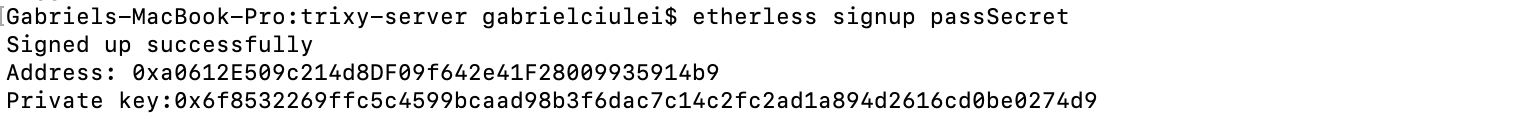
\includegraphics[width=\textwidth]{res/img/signup.png}
		\caption{Signup command}
	\end{figure}\\
\subsubsection{Login}
If an account already exists and the intent is to use it for Etherless, then the private key can be used to login using the following command:\\\\
\centerline{\code{etherless login <privateKey> <password>}}\\\\
The password is a user-chosen string that will be used to encrypt your credentials locally.\\\\
\textbf{Attention!} The account address is not necessary because it can be deducted from the private key.\\\\
\begin{figure}[h]
	\begin{center}
	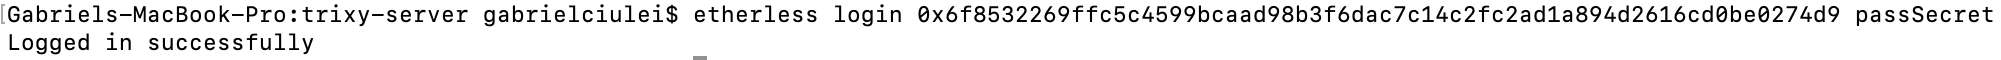
\includegraphics[width=\textwidth]{res/img/login.png}
	\caption{Login command}
	\end{center}
\end{figure}
\subsubsection{Logout}
To disconnect the currently logged account, use the following command:\\\\
\centerline{\code{etherless logout}}\\\\
This command will remove all session data and encrypted stored credentials. The password used during login or registration now becomes useless. To be able to use again Etherless functionalities, you will need to login again or generate a new account.\\
\begin{figure}[h]
	\centering
	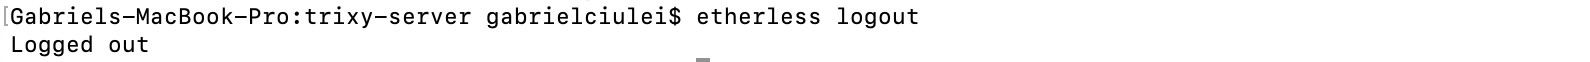
\includegraphics[width=\textwidth]{res/img/logout.png}
	\caption{Logout command}
\end{figure}
\newpage
\subsection{Commands guide}
\subsubsection{List}
This command will show you a list of all functions that have been uploaded to Etherless by its users and it's used as follows:\\\\
\centerline {\code{etherless list}}\\\\
For each function found, the following data is displayed:
\begin{itemize}
	\item \textbf{NAME}: the name of the function which is used to uniquely identify it (eg. for execution request);
	\item \textbf{COST}: the fee detracted from the account each time execution is requested;
	\item \textbf{PROTOTYPE}: a description of the parameters the functions needs;
	\item \textbf{DESCRIPTION}: a textual function description.
\end{itemize}
Example:
\begin{figure}[h]
	\begin{center}
	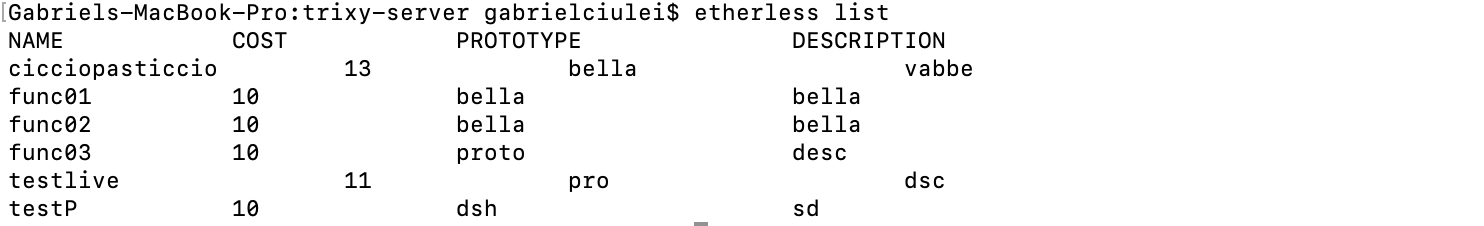
\includegraphics[width=\textwidth]{res/img/list.png}
	\caption{List command}
	\end{center}
\end{figure}
\subsubsection{Find}
Retrieves information about a given function and it's used as follows:\\\\
\centerline {\code{etherless find <functionName>}}\\\\
The following data is displayed for the searched function:
\begin{itemize}
	\item \textbf{NAME}: the name of the function which is used to uniquely identify it (eg. for execution request);
	\item \textbf{COST}: the fee detracted from the account each time execution is requested;
	\item \textbf{PROTOTYPE}: a description of the parameters the functions needs;
	\item \textbf{DESCRIPTION}: a textual function description;
	\item \textbf{OWNER}: a textual function description.
\end{itemize}
Example:
\begin{figure}[h]
	\begin{center}
	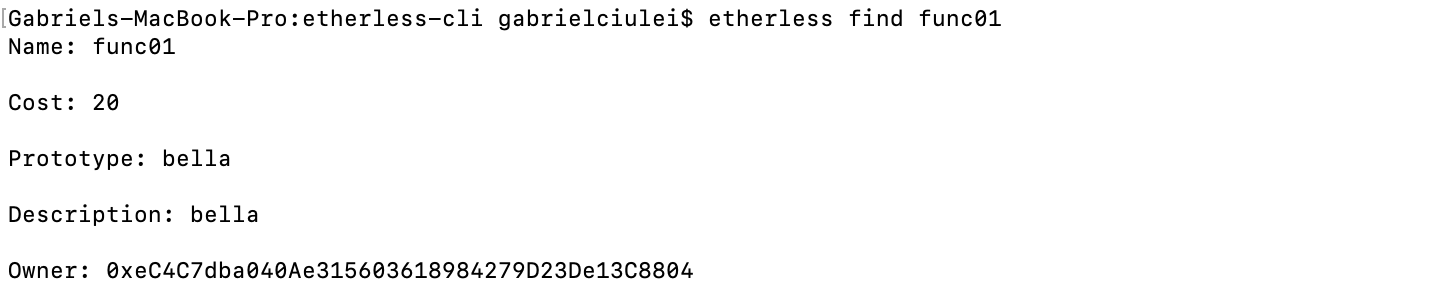
\includegraphics[width=\textwidth]{res/img/find.png}
	\caption{Find command}
	\end{center}
\end{figure}

%\subsubsection{Find}
%The user can search informations about a %specific function already deployed\glo by %another developer, typing the function %name.\\\\
%\centerline{\code{find <function name>}}
%\begin{figure}
%	\centering
%	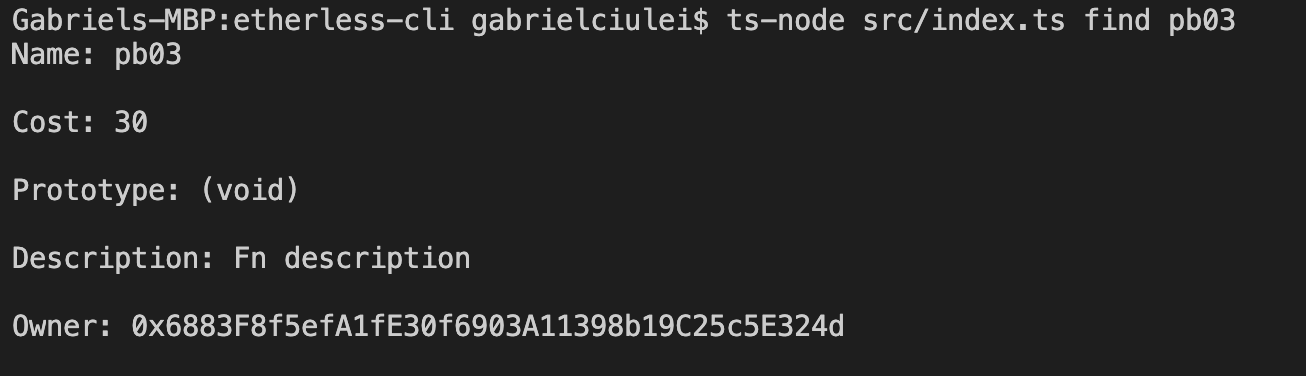
\includegraphics[width=\textwidth]{res/img/Screenshot_find.jpg}
%	\caption{Find command}
%\end{figure}
%\\
%\\aggiungere screen comando
%\subsubsection{Log}
%The user can retrieve all the information about the latest transactions through the command "log".\\\\
%\centerline{\code{log}
%\begin{figure}
%	\centering
%	\includegraphics[width=\textwidth]{res/img/Screenshot_log.jpg}
%	\caption{Log command}
%\end{figure}}
%aggiungere screen comando
\subsubsection{Create}
This command is used to request execution of a remote function. This is a synchronous command. Once launched it returns the result of the function or, in case the functions have some execution issues, an exception.\\\\
\centerline{\code{etherless create <functionName> <description> <prototype> <cost> <functionFile> <password>}}\\\\
\\\\
Input parameters are:
\begin{itemize}
	\item \textbf{functionName [string]}: a string containing the name of the function;
	\item \textbf{description [string]}: a string containing the description of the function;
	\item \textbf{prototype [string]}: a string containing the description of the parameters that uploaded function takes in;
	\item \textbf{functionName [int]}: the fee amount (in wei) you wish to receive when your function is used; on top of this amount, service fees will be added;
	\item \textbf{functionFile [path]}: a path to the file containing the function;
	\item \textbf{password [string]}: the password you set up during signup/login.
\end{itemize}
\textbf{Attention!} JavaScript\glo function needs to be properly formatted so that the system is then able to interface with it.\\\\
\textbf{Note!} A template function is provided (./prima.js).\\\\
Example:
\begin{figure}[h]
	\centering
	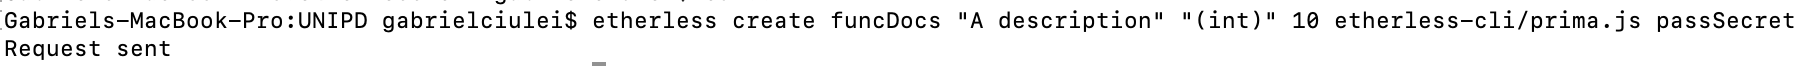
\includegraphics[width=\textwidth]{res/img/create.png}
	\caption{Create command}
\end{figure}

\subsubsection{Run}
This command is used to request execution of a remote function. This is a synchronous command. Once launched it returns the result of the function or, in case the functions have some execution issues, an exception.\\\\
\centerline{\code{etherless run <functionName> <password> [parameters...]}}\\\\
\\\\Other than the name of the the function to be run, password and parameters are necessary. Since the execution of the function will consume credit from your account, the private key needs to be accessed. Function parameters should be passed as function prototype instructs.\\\\
\textbf{Attention!} The parameters passed to the function need to mirror prototype description, otherwise an error will probably occur.\\\\
Example:
\begin{figure}
	\centering
	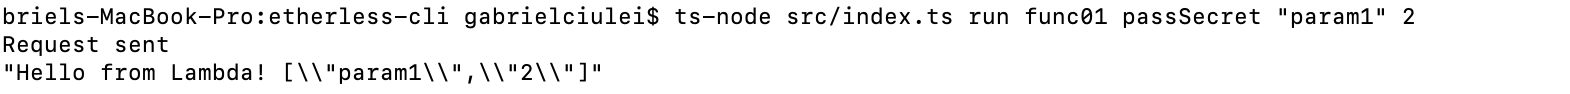
\includegraphics[width=\textwidth]{res/img/run.png}
	\caption{Run command}
\end{figure}
\subsubsection{Set}
This command is used to update a function property.\\\\
\centerline {\code{etherless set <functionName> <property> <newValue> <password>}}\\\\
The target function to update is identified by \textit{function name}. Only the owner of the function can update function properties.\\\\
Properties that can be updated are the following:
\begin{itemize}
	\item \textbf{description}: to update the function description;
	\item \textbf{cost}: to update the function cost for execution;
	\item \textbf{prototype}: to update the function prototype.
\end{itemize}
Example:
\begin{figure}[h]
	\begin{center}
	
\includegraphics[width=\textwidth]{res/img/set.png}
	\caption{Set command}
	\end{center}
\end{figure}
\subsubsection{Update}
Updates the code of an already existing function:\\\\
\centerline {\code{etherless update <functionName> <functionFile> <password>}}\\\\
\textit{Function file} will contain a path to the function file on the file system.\\
A user can only update his own functions. Further requests for function execution will result in usage of the new uploaded code.\\
Example:
\begin{figure}[h]
	\begin{center}
	
\includegraphics[width=\textwidth]{res/img/update}
	\caption{Update command}
	\end{center}
\end{figure}
\subsubsection{Delete}
Deletes a function from the service:\\\\
\centerline {\code{etherless delete <functionName> <password>}}\\\\
A user can only delete his own functions. Further requests for a deleted function will result in an error.\\
Example:
\begin{figure}[h]
	\begin{center}
	
\includegraphics[width=\textwidth]{res/img/delete}
	\caption{Delete command}
	\end{center}
\end{figure}
\subsubsection{Log}
Shows a list of all execution requests a user has taken in the past on his machine.\\\\
\centerline {\code{etherless log}}\\\\
Shows a list of past execution requests. The following data is displayed for each log row:
\begin{itemize}
	\item \textbf{name}: the name of the function requested;
	\item \textbf{cost}: execution cost for function request;
	\item \textbf{datetime}: execution date and time for requested function;
\end{itemize}
Example:
\begin{figure}[h]
	\begin{center}
	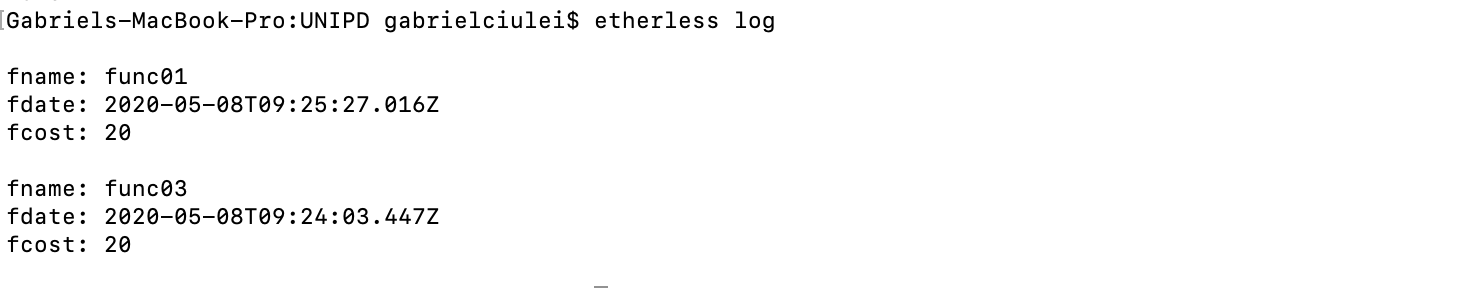
\includegraphics[width=\textwidth]{res/img/log.png}
	\caption{Log command}
	\end{center}
\end{figure}
